\documentclass{ieeeaccess}
%\usepackage{cite}
\usepackage{amsmath,amssymb,amsfonts}

%\usepackage{algorithmic}
%\usepackage{algorithm}
%\usepackage{algpseudocode}
\usepackage{graphicx}
\usepackage{textcomp}
\usepackage[utf8]{inputenc}

\usepackage[backend=biber, style=ieee]{biblatex}
\addbibresource{references.bib} % conecta o arquivo externo

\usepackage[T1]{fontenc}
\usepackage{lmodern} % Or \usepackage{cm-super}

\usepackage{booktabs}
\usepackage{siunitx}

\usepackage{comment}

\usepackage{bm}
\makeatletter
\AtBeginDocument{\DeclareMathVersion{bold}
\SetSymbolFont{operators}{bold}{T1}{times}{b}{n}
\SetSymbolFont{NewLetters}{bold}{T1}{times}{b}{it}
\SetMathAlphabet{\mathrm}{bold}{T1}{times}{b}{n}
\SetMathAlphabet{\mathit}{bold}{T1}{times}{b}{it}
\SetMathAlphabet{\mathbf}{bold}{T1}{times}{b}{n}
\SetMathAlphabet{\mathtt}{bold}{OT1}{pcr}{b}{n}
\SetSymbolFont{symbols}{bold}{OMS}{cmsy}{b}{n}
\renewcommand\boldmath{\@nomath\boldmath\mathversion{bold}}}
\makeatother


%Your document starts from here ___________________________________________________
\begin{document}
\history{Date of publication xxxx 00, 0000, date of current version xxxx 00, 0000.}
\doi{10.1109/ACCESS.2024.0429000}

\title{Context-oriented Synthesis of Salt Domes in Labeled Seismic Images}
\author{\uppercase{Luciano D. Terres}\authorrefmark{1} and
\uppercase{Jacob Scharcanski}\authorrefmark{2}, \IEEEmembership{Senior Member, IEEE} }

\address[1]{Institute of Informatics,
Federal University of Rio Grande do Sul, Porto Alegre, RS, Brasil, 91501-970, e-mail: ldterres@inf.ufrgs.br}
\address[2]{Institute of Informatics, 
Federal University of Rio Grande do Sul, Porto Alegre, RS, Brasil, 91501-970, e-mail: jacobs@inf.ufrgs.br}

\markboth
{Author \headeretal: Preparation of Papers for IEEE TRANSACTIONS and JOURNALS}
{Author \headeretal: Preparation of Papers for IEEE TRANSACTIONS and JOURNALS}

\corresp{Corresponding author: Jacob Scharcanski (e-mail: jacobs@inf.ufrgs.br).}


\begin{abstract}
Advanced remote sensing and seismic image interpretation methods often rely on large annotated datasets for training robust advanced machine learning models. However, in practice, obtaining such large training datasets can be hard in applications such as offshore oil exploration. Besides, expert annotation of large seismic image datasets can be costly and demanding. This work proposes a new seismic image data augmentation method focused in the context of images containing saline dome rocks, by artificially generating seismic image data containing saline rocks, as well as their mask labels at pixel level. A combination of variational autoencoders (VAE) and texture synthesis algorithms is used to generate synthetic labeled samples. VAEs are used to learn real rock geometries and generate new ones with annotated correspondent mask information. The masks will drive a non-parametric texture synthesizer of seismic images. The experimental results were validated by experts and suggest that the proposed methodology can be used efficiently to increase the number of seismic images samples. 
\end{abstract}

\begin{keywords}
Data augmentation, deep learning, image segmentation, seismic images, seismic interpretation, texture synthesis, and variational autoencoders.
\end{keywords}

\titlepgskip=-21pt

\maketitle

\section{Introduction}
\label{sec:introduction}
\PARstart{A} relevant task in seismic imaging and interpretation is to distinguish accurately saline bodies from other sediments. However, seismic reflections in salt rocks poses a challenge to seismic imaging researchers due to their distinct acoustic characteristics and complex geometry.  The boundaries of saline bodies can be identified by trained experts \cite{ref5}, but involve massive amounts of data and such task is labor intensive, making this task a potentially candidate for being handled by smart image segmentation methods. Nevertheless, public databases of annotated seismic images are scarce, and such data is needed for training of seismic image segmentation methods. deep neural networks, such as RESNET and UNET, specialized in image segmentation and recognition. Therefore, researchers recently have directed their efforts towards data augmentation by seismic image synthesis \cite{ref1}.

In this work, a mechanism for synthesizing annotated seismic image samples containing salt domes is proposed. A combination of a variational autoencoder (VAE) neural network and a context-oriented texture synthesis method is used to generate new seismic image samples. The VAE is a  multilayer neural networks containing an encoder and a decoder. The VAE encoder maps the multidimensional seismic image into a low-dimensional deep feature space. Then, the decoder maps the deep features back into the image space to reconstruct the seismic image. The objective is to minimize the difference between the input data and the reconstructed (synthesized) image samples \cite{ref3}.

Visual texture synthesis can learn how to generate new seismic samples of a particular seismic image by inferring its generation process from examples. The generated (synthesized) seismic textures should be indistinguishable from real natural seismic data from the human experts point of view. If the experts cannot distinguish between an original seismic texture and a synthesized one, the synthesis process is considered successful \cite{ref4}. This work innovates by combining VAEs to generate the salt and rock shapes and by creating a context for the seismic texture synthesis process, which can work with non-stationary seismic image textures of salt bodies, conventional rocks, and their boundaries. 

\section{Fundamentals and Literature Review}

 \PARstart{I}{n} the early days, before the rise of neural networks, researchers relied on traditional methods like model-based approaches and basic texture synthesis techniques. These methods worked reasonably well for simple tasks but often struggled with complex geological features and non-uniform textures commonly found in seismic data. The primary limitation of these early techniques was their inability to handle non-stationary textures, which are textures that change across different regions of an image \cite{ref16}.

 Over the past decades, a broad spectrum of algorithms has been proposed to address the challenges in seismic image synthesis. In recent years, the adoption of deep learning techniques has significantly advanced the field \cite{ref5}. The introduction of neural networks around 2010 marked a major turning point. Convolutional Neural Networks (CNNs), in particular, brought a new level of sophistication to seismic image synthesis. CNNs excel at extracting detailed features from images, such as horizontal and vertical lines, and can even complete entire objects within an image. This capability allowed for more accurate and realistic seismic images, enabling better interpretation of subsurface structures \cite{ref14}. 

However, the success of CNNs came with a significant challenge: these learning structures require large, annotated datasets for training. In seismic imaging, such datasets tend to be unavailable or difficult to produce. Therefore, researchers have explored various alternatives,  including data augmentation with synthetic data and transfer learning. Despite these efforts, the issue of limited training data remains a hurdle in the widespread application of CNNs to seismic image synthesis \cite{ref15}.

In 2020, R. S. Ferreira et al. \cite{ref19}  proposed similar work for generating synthetic seismic images. In addition to using expert evaluation, they also evaluated their results using metrics that estimate the distance between synthetic and real images. The article addresses the generation of synthetic seismic images of various geological fields, including geological faults and salt domes. In this sense, we compare the results using the same metrics and methodologies, evaluating the realism of synthetic seismic images when contrasted to real images.

Henriques et al. \cite{ref1} proposed a very similar Data Augmentation method based on training two generative models to augment the number of samples in a seismic image dataset for the semantic segmentation of salt bodies. However, they perform an indirect evaluation of results, based on the improvement in the performance of segmentation methods based on convolutional neural networks, which could be difficult to use as a direct comparison of results with our proposed method and a different database.

\section{Proposed Methodology}

The Context-Oriented Seismic Image Synthesis methodology combines a deep learning model based on VAE with a texture synthesis algorithm. It generates seismic image samples for data augmentation within a specific context mask, as outlined below. The convolutional neural network is a variational auto-encoder model (VAE) that generates salt body masks corresponding to a given salt geometry. Using the generated mask geometry, a new image is synthesized using a non-parametric texture synthesis algorithm. The proposed method focuses on context zones and on the characteristics of seismic images with salt domes. %A schema of the proposed method is presented in Algorithm.  ~\ref{alg:alg1}.


\subsection{Context Generation Using a Variational Autoencoder}

The proposed data augmentation scheme detects and generates new rock geometries with a Variational Autoencoder, as shown in Fig.~\ref{fig:vae1}.  
\begin{figure}
    \centering
    \includegraphics[width=1\linewidth]{images/vaesGen.png}
    \caption{Samples of generated structural salt masks. The Variational Autoencoder learns the distribution and reproduce new structural masks.}
    \label{fig:vae1}
\end{figure}

A dataset of seismic images used to generate new salt masks is illustrated in Fig. \ref{fig:vae1}. The natural intersection between two different rocks are their boundaries, and in the case of salt rock this boundary is usually apparent, as seen in Fig. \ref{fig:edge1}. During the VAE training process, only salt masks with a considerable amount of salt are used, varying from 10 to 90 percent of the total area.
\begin{figure}
    \centering
    \includegraphics[width=1\linewidth]{images/edge detection.png}
    \caption{Sample of the boundaries identification between salt and other sediments represented in a dilated edge segment.}
    \label{fig:edge1}
\end{figure}

The generated masks are used as contexts for the seismic texture synthesis process. Once the boundaries of a salt body are known, the region interior to the closed boundary is expected to be salt. Auto-Encoding Variational Bayes, commonly known as Variational Autoencoders (VAEs), is a deep learning technique~\cite{ref8} used in this work as a generative model for learning a probabilistic mapping from an input space to a latent space and back, allowing data reconstruction and new data generation. The VAE model used is a simple feedforward network for the encoder and decoder. The encoder contains four stacked dense layers, and the decoder contains five stacked dense layers. During the inference time, the latent variables $z$ are sampled from the prior distribution $\pi(z)$, and then $z$ is decoded with the VAE´s decoder to generate the salt mask with the inferred distribution.

The main task of VAEs is to model the underlying probability distribution of a data set $\mathbf{x} = \{x^{(1)}, x^{(2)}, \ldots, x^{(N)}\}$. The model introduces a latent variable $\mathbf{z}$ obtained by maximizing the marginal likelihood:

\begin{equation}
p_\theta(x) = \int p_\theta(x | z) p(z) \, dz
\end{equation}
The key VAE components are the following :

\paragraph{Encoder (Recognition Model)}
Maps an input $x$ to a latent variable $z$, and approximates the posterior distribution $q_\phi(z | x)$ assuming it is Gaussian:

\begin{equation}
q_\phi(z | x) = \mathcal{N}(z; \mu_\phi(x), \Sigma_\phi(x))
\end{equation}
where $\mu_\phi(x)$ and $\Sigma_\phi(x)$ are the posterior distribution $q_\phi(z | x)$ mean and the covariance, that are outputs of the encoder network.

\paragraph{Decoder (Generative Model)}
Reconstructs the data from the latent variable $z$, modeling the likelihood $p_\theta(x | z)$ assuming it as Gaussian:

\begin{equation}
p_\theta(x | z) = \mathcal{N}(x; \mu_\theta(z), \Sigma_\theta(z))
\end{equation}

where $\mu_\theta(z)$ and $\Sigma_\theta(z)$ are the posterior distribution $q_\phi(z | x)$ mean and the covariance, that are outputs of the decoder network.

\paragraph{Latent Variables Priors $p(z)$}
Usually assumed as a standard normal distribution:

\begin{equation}
p(z) = \mathcal{N}(z; 0, I)
\end{equation}

where $I$ is the identity matrix.

\paragraph{Variational Inference} Since the exact posterior $p(z | x)$ is intractable, VAEs use variational inference to approximate it by optimizing the evidence lower bound (ELBO):

\begin{equation}
\log p_\theta(x) \geq \mathbb{E}_{q_\phi(z | x)} \left[ \log p_\theta(x | z) \right] - \text{KL}(q_\phi(z | x) \parallel p(z)),
\end{equation}
and the ELBO has two important components: reconstruction loss, and (KL) divergence loss, which are detailed next. The reconstruction loss is the expected log-likelihood of the data, which encourages an accurate sample reconstruction:

\begin{equation}
\mathbb{E}_{q_\phi(z | x)} \left[ \log p_\theta(x | z) \right]
\end{equation}
and the KL divergence loss is the Kullback-Leibler divergence between the approximate posterior and the prior, which acts as a regularizer:

\begin{equation}
\begin{aligned}
\text{KL}(q_\phi(z | x) \parallel p(z)) 
=  \\
\frac{1}{2} \sum_{i=1}^{d} \left( \mu_\phi(x)_i^2 + \Sigma_\phi(x)_{ii} - \log \Sigma_\phi(x)_{ii} - 1 \right)
\end{aligned}
\end{equation}

where $d$ is the dimensionality of the latent space.

In order to enable the gradient-based optimization, the reparameterization trick is used so instead of sampling $z \sim q_\phi(z | x)$ directly, $z$ is expressed as:

\begin{equation}
z = \mu_\phi(x) + \Sigma_\phi(x)^{1/2} \odot \epsilon, \quad \epsilon \sim \mathcal{N}(0, I)
\end{equation}
allowing for gradients to be propagated through $\mu_\phi(x)$ and $\Sigma_\phi(x)$ by treating $\epsilon$ as an auxiliary variable.

Finally, VAEs are trained by maximizing the ELBO with respect to the parameters $\theta$ and $\phi$ using stochastic gradient descent. The optimization process balances reconstruction accuracy with latent space regularization.

\subsection*{Advantages of Variational Autoencoders}
The primary reasons for using VAEs are a realistic generation of synthetic samples, an increase in dataset diversity, a regularization and control of variability, and an improvement in the generalization of the segmentation model. Considering specific reasons related to the nature of seismic data and the purpose of sample generation for data augmentation, VAEs enable the generation of synthetic images that preserve the structural characteristics of real seismic data, thereby enhancing the training and performance of segmentation models \cite{ref1} \cite{ref15} \cite{ref18}.

\subsection*{Comparison with Generative Adversarial Networks (GANs)}

\begin{enumerate}
    \item \textbf{Control over Data Variability}:
    \begin{itemize}
        \item It is essential that the generated images preserve the structural patterns of salt bodies. VAEs ensure that synthetic images fall within the expected distribution of real seismic images. GANs, on the other hand, are more prone to generating images with high variability and may occasionally create unrealistic or inconsistent samples \cite{ref16}.
    \end{itemize}
    \item \textbf{Regularization and Smoothness in Image Generation}:
    \begin{itemize}
        \item VAEs impose a probabilistic structure on the latent space, resulting in smoother transitions between different samples and generating images that maintain coherent structural characteristics. GANs, in turn, can suffer from mode collapse \cite{ref16}, where they generate only a limited subset of possible data variations, reducing the diversity of the augmented dataset.
    \end{itemize}
    \item \textbf{Training Stability}:
    \begin{itemize}
        \item GANs require a balance between the generator and discriminator, which can make training unstable and more challenging to converge to a distribution that well represents the seismic data \cite{ref16}.
    \end{itemize}
\end{enumerate}

Although GANs are known for generating high-quality images, VAEs were chosen in this work due to their more refined control over data variability, training stability, and preservation of the latent seismic data distribution.

\subsection*{Disadvantages of Diffusion Models}
Conversely, diffusion models present practical and conceptual disadvantages \cite{ref17}:
\begin{enumerate}
    \item \textbf{Higher Computational Cost}:
    \begin{itemize}
        \item Diffusion models require many sampling steps to generate images, typically hundreds or thousands of denoising steps \cite{ref17}. This makes them more computationally expensive than VAEs, which generate samples in a single pass through the model.
        \item In seismic applications, where there is a need to generate a large number of samples for data augmentation, the efficiency of VAEs can be a significant advantage. 
    \end{itemize}
    \item \textbf{Need for Large Volume of Training Data}:
    \begin{itemize}
        \item Diffusion models often require large training datasets to capture high-quality distributions  \cite{ref17}. Since labeled seismic images can be limited, VAEs may be more effective in learning useful representations even with a smaller number of samples.
    \end{itemize}
\end{enumerate}

Therefore, targeting efficiency and ease of training, VAEs have simpler and more stable training, as they do not rely on an iterative refinement process like diffusion models. This can be a decisive factor when there are time and computational resource constraints.

\begin{comment}
\begin{algorithm}[H]
\caption{Seismic Image Synthesis Algorithm}\label{alg:alg1}
\begin{algpseudocode}
\begin{enumerate}
    \State \textbf{Data Preparation}
    \State \textbf{Training the Variational Autoencoder Model}
    \State \textbf{Generating New Salt Body Masks}
    \State \textbf{Contextual Data Augmentation}
    \State \textbf{Texture Synthesis Context-oriented}
    \State \textbf{Final Sample Output}
\end{enumerate}
\end{algpseudocode}
\end{algorithm}
\end{comment}


\subsection{Non-Parametric Context-oriented Texture Synthesis}

The typical texture synthesis algorithms use an image database and replicate the images in a picture plane according to some arrangement rules. The texture synthesis can be enhanced by working at a finer scale, from the pixel level to a small region level. At each iteration of the algorithm, a small section of the original texture, a patch, is copied and placed within the newly synthesized texture. Non-parametric sampling \cite{ref12} improved further texture synthesis by creating a new image that shares the same statistical properties as a given sample texture, while avoiding explicit models of the texture by directly sampling from example images.

The proposed seismic texture synthesis method requires the following components:

\textbf{1. Neighborhood Definition:} For each pixel $p$ in the image to be synthesized, a region around $p$ already filled with known values is defined (namely, a neighborhood $N(p)$;

\textbf{2. Similarity Criterion:} To find a corresponding patches in the example image, the similarity between $N(p)$ and the neighborhoods $N(q)$ are computed for all pixels $q$ in the example image. A similarity measure is defined as the Euclidean distance between the pixels of the neighborhoods:

\begin{equation}
D(N(p), N(q)) = \sum_{i \in N} \left( I_p(i) - I_q(i) \right)^2,
\end{equation}
where $I_p(i)$ and $I_q(i)$ are the pixel values at the image locations $i$ in the neighborhoods of $p$ and $q$, respectively;

\textbf{3. Random Sampling:} A pixel $q$ is chosen randomly from the example image with probability proportional to its similarity (or inverse of $D(N(p), N(q))$) to $p$. In other words, pixels with smaller $D(N(p), N(q))$ are more likely to be chosen. The probability of choosing a pixel $q$ can be modeled as:

\begin{equation}
P(q) = \frac{\exp(-D(N(p), N(q)) / \sigma^2)}{\sum_{q'} \exp(-D(N(p), N(q')) / \sigma^2)}
\end{equation}
where $\sigma$ controls the influence of distances on the pixel $q$ selection probability;

\textbf{4. Image Filling:} The process begins with a small initial patch in the new image and gradually expands it, pixel by pixel, using the steps described above to fill the entire image. The choice of the next pixel to be synthesized follows a raster or spiral filling path. The method produces seismic textures that are visually similar to the original input texture. 

Next, the process of seismic image synthesis is detailed. Various patches are used as inputs. These patches correspond to different parts of the seismic image and are based on the context mask generated by the VAE model. The synthesized sample has three main components, namely, salt zone, boundary zone, and conventional rock zone. Initially, the boundary, or frontier, zones between the two rocks, which also is called edge zone, is  created. The boundary zones is created by using edge detection to identify the interface between the two types of rocks, and to make it thicker, creating an edge strip. As seeing in Fig.\ref{fig:edge1}, this strip is an area of high seismic contrast appearing as light and dark bands. Also, there are various parallel lines that make up this boundary, and their angles can be seen in Fig. \ref{fig:line1}. A dataset composed of edges pieces and their corresponding angles is used as input for the boundary synthesis process. Then, for each edge segment in the mask of the image to be synthesized, its texture is synthesized based on the patch with the most similar angle (see Fig.\ref{fig:edge2}). This process is repeated until all the segments of the edge band are covered.

\begin{figure}
    \centering
    \includegraphics[width=1\linewidth]{images/7.png}
    \caption{The Green lines at original image identify border zones and angles to orient the patch selection for patch database construction process.}
    \label{fig:line1}
\end{figure}

\begin{figure}
        \centering
        \includegraphics[width=1\linewidth]{images/edge3.jpg}
        \caption{The Construction of new boundaries in generated images uses  texture sinthesys over selected samples from patch database.}
        \label{fig:edge2}
    \end{figure}    

In order to synthesis the salt zones, the corresponding source image region is used as a seismic texture reference to generate new synthesized pixels. Finally, the conventional rock zone is synthesized using the corresponding sediment regions in the source sample. The seismic image synthesis is divided in steps to conform to the specific characteristics of this kind of image, such as the edge, saline rock, conventional rock zones, as seen in Fig. \ref{fig:source1}. Similarly, the algorithm processes all zones, one by one, to complete the seismic image synthesis process using their corresponding zone samples in the input data.

\begin{figure}
    \centering
    \includegraphics[width=1\linewidth]{images/2.png}
    \caption{Real seismic saline images divided by context zones as input to the texture synthesis process.}
    \label{fig:source1}
\end{figure}


\section{Experimental Results and Evaluation}

The enhancement of the proposed approach can be demonstrated through qualitative and quantitative evaluations comparing the results of the method with existing state-of-the-art techniques. The article demonstrates the effectiveness of the model by the following criteria:

\begin{enumerate}
    \item \textbf{Qualitative Evaluation by Experts}: Experts try to identify the portions of salt dome structures inside the seismic samples. The expert produces a mask label that will be compared with the ground truth mask. Quantitative metrics, such as the F1 score, are used to evaluate the difference between the expert prediction and the ground truth. 
    
    \item \textbf{Quantitative Comparison with Related Work}:
    A very similar work In “Generating Sketch-Based Synthetic Seismic Images With Generative Adversarial Networks” \cite{ref19}, use the metrics mean squared error (MSE), structural similarity (SSIM) and Euclidean distance based on the Local Binary Pattern (LBP) to measure texture attributes between original seismic sketches and the samples synthesized by the networks. We will evaluate the samples generated by our proposed method with the same metrics and compare the results.
\end{enumerate}

\subsection{Dataset}

The salt body dataset was obtained from the TGS Salt Identification Challenge, a machine learning competition on Kaggle. It comprises 2D image slices representing a 3D view of the Earth's interior obtained through reflection seismology. The data is a set of images chosen randomly in the subsurface. The photos are 101 x 101 pixels and each pixel is classified as either salt or sediment \cite{ref13}. 

\begin{figure}
    \centering
    \includegraphics[width=1\linewidth]{images/fig8.png}
    \caption{Comparison between real sample, geoscience specialist selection over saline area and ground truth (saline mask).}
    \label{fig:expert1}
\end{figure}



\subsection{Evaluation Metrics}

Through qualitative analysis, the geoscience specialist evaluates the samples to identify the portions of salt bodies in the seismic images. To assess the quality of generation , the metrics precision, recall, and F1-score compare the synthetic seismic image with the ground truth, as detailed below:

The F1 score is a widely used measure for evaluating binary classification models. It is particularly useful when a balance between precision and recall is desired. It allows access to the quality of the classification predictions. While the correct classification rate is simple to understand, it can be misleading in imbalanced datasets. Therefore, measures such as precision, recall, and the F1 score tend to provide a clearer scenario \cite{ref14}.

\begin{itemize}
    \item \textbf{Precision:} is the proportion of true positives (TP) over all predicted positive results (TP + FP).
    \begin{equation}
    \text{Precision} = \frac{TP}{TP + FP}
    \end{equation}

    \item \textbf{Recall:} or sensitivity, is the proportion of true positives over all actual positive cases (TP + FN).
    \begin{equation}
    \text{Recall} = \frac{TP}{TP + FN}
    \end{equation}


    \item \textbf{F1 Score:} is the harmonic mean of precision and recall, providing a single metric that considers both. 

\end{itemize}
    \begin{equation}
    \text{F1 Score} = 2 \times \frac{\text{Precision} \times \text{Recall}}{\text{Precision} + \text{Recall}}
    \end{equation}
    
 The F1 score is particularly valuable in classification situations where the positive class is rare. It helps to understand the trade-off between false positives and false negatives. In several practical applications, the F1 score provides a balanced measure that is less susceptible to class distribution bias.

The precision, recall, and F1-score measures are used for evaluating the salt bodies masks generated by the experts, and can be computed using the confusion matrix derived from these experts generated masks. To evaluate the quality of the synthesized samples, the overlap between the experts selections of pixels corresponding to the salt bodies in synthetic images, and synthetic images masks is evaluated, as shown in Fig. \ref{fig:expert1}.

Fig. \ref{fig:expert2} illustrates the ground truth image and the specialist evaluation of the salt bodies locations, and the computed precision, recall, and F1-score measures for this particular case.

Related to a quantitative comparison, following "Generating Sketch-Based Synthetic Seismic Images With Generative Adversarial Networks" \cite{ref19}, we assess the quality of the produced samples by comparing each synthetic image with the original seismic image that serves as a template. The template is the basis for producing the sketches that guide the samples' production. To this end, we use the metrics mean squared error (MSE), Structural Similarity Index (SSIM), and Euclidean distance based on the Local Binary Pattern (LBP) texture attribute between the original seismic image that serves as a template for sketch production and the synthetic images.

The Mean Squared Error (MSE) defines a pixel-to-pixel distance between two images. We calculate it as follows: subtract each synthetic pixel value from the real one. Square each error: this eliminates negative signs and penalizes larger errors. Finally, take the average of these squares as seen in equation \ref{eq:mse}.

\begin{equation}
\label{eq:mse}
\text{MSE} = \frac{1}{n} \sum_{i=1}^{n} (y_i - \hat{y}_i)^2
\end{equation}

The SSIM is a metric that measures the perceptual similarity between two images by incorporating some texture information, such as variances and covariances. It is widely used in computer vision and image processing to assess the quality of image reconstructions, compressions, or transmissions. It evaluates luminance (brightness), contrast, and structural attributes as local patterns and shapes. Since SSIM values are defined in the range [-1, 1], the common transformation \ref{eq:mse2} represents it as a distance to facilitate comparison, and from now on, it is called DSSIM.

\begin{equation}
\label{eq:mse2}
\text {DSSIM(x, y)= (1 - SSIM(x, y))/2}
\end{equation}

The interpretation of DSSIM values as a distance between 0 and 1 is as follows: 

\begin{itemize}
    \item DSSIM = 0: the images are identical
    \item DSSIM from 0,005 to 0.10: high similarity
    \item DSSIM > 0.25: low perceptual similarity
    \item DSSIM from 0,5 to 1: very different
\end{itemize}

The LBP is a more robust texture attribute successfully applied in medical images and geosciences \cite{vatamanu_content-based_2013}, \cite{britto_mattos_assessing_2017}. The LBP calculation here uses four neighbors, distance 1, and a 64-pixel tile size. The calculation produces a histogram for each image, representing the frequency of local binary patterns. Finally, we compute the Euclidean Distance between the histograms. Therefore, the smaller the distance, the more similar the textures of the two images are. Otherwise, larger histogram distances represent different patterns.

\begin{figure*}
    \centering
    \includegraphics[width=1\textwidth]{images/imagens.png}
    \caption{Synthetic Seismic Samples}
    \label{fig:placeholder}
\end{figure*}


\begin{figure}
    \centering
    \includegraphics[width=1\linewidth]{images/expert.png}
    \caption{Quantitative analisys demonstration: Sample measurement between groud truth and expert analisys: Precision: 0.88 ; Recall: 0.87 ; F1-score: 0.87.}
    \label{fig:expert2}
\end{figure}

\begin{table*}[h!]
\centering
\caption{Result table: real images evaluation by the experts.}
\label{tab:real_images_evaluation}
\begin{tabular}{|c|c|c|c|c|c|c|c|c|c|c|}
\hline
\multicolumn{11}{|c|}{\textbf{Database Real Images}} \\
\hline
~ & \multicolumn{3}{c|}{\textbf{Expert 1}} & \multicolumn{3}{c|}{\textbf{Expert 2}} & \multicolumn{3}{c|}{\textbf{Expert 3}} & \textbf{Mean} \\
\cline{2-11}
\textbf{Metrics} & \textbf{Precision} & \textbf{Recall} & \textbf{F1-score} & \textbf{Precision} & \textbf{Recall} & \textbf{F1-score} & \textbf{Precision} & \textbf{Recall} & \textbf{F1-score} & \textbf{F1-score} \\
\hline
Standard Deviation & 0,06034 & 0,04584 & 0,04037 & 0,05429 & 0,04763 & 0,04408 & 0,04780 & 0,05288 & 0,03414 & 0,03953 \\
\hline
Mean & 0,91480 & 0,91563 & 0,91396 & 0,91845 & 0,90420 & 0,91064 & 0,82958 & 0,81400 & 0,82017 & 0,88159 \\
\hline
\end{tabular}
\end{table*}

\begin{table*}[h!]
\centering
\caption{Result table: Synthetic images evaluation by the experts.}
\label{tab:synthetic_images_evaluation}
\begin{tabular}{|c|c|c|c|c|c|c|c|c|c|c|}
\hline
\multicolumn{11}{|c|}{\textbf{Synthetic Samples}} \\
\hline
~ & \multicolumn{3}{c|}{\textbf{Expert 1}} & \multicolumn{3}{c|}{\textbf{Expert 2}} & \multicolumn{3}{c|}{\textbf{Expert 3}} & \textbf{Mean} \\
\cline{2-11}
\textbf{Metrics} & \textbf{Precision} & \textbf{Recall} & \textbf{F1-score} & \textbf{Precision} & \textbf{Recall} & \textbf{F1-score} & \textbf{Precision} & \textbf{Recall} & \textbf{F1-score} & \textbf{F1-score} \\
\hline
Standard Deviation & 0,06706 & 0,04698 & 0,04509 & 0,05597 & 0,05397 & 0,04433 & 0,05221 & 0,05644 & 0,03889 & 0,04277 \\
\hline
Mean & 0,90439 & 0,89575 & 0,89868 & 0,88823 & 0,87772 & 0,88186 & 0,83354 & 0,82261 & 0,82648 & 0,86901 \\
\hline
\end{tabular}
\end{table*}



\begin{table}[h!]
\centering
\caption{Statistics for sinthesys group \texttt{0bdd44d530} with 100 images}
\resizebox{0.5\textwidth}{!}{%
\begin{tabular}{|l|c|c|c|c|c|c|}
\hline
\textbf{Metric} & \textbf{Min} & \textbf{Q1} & \textbf{Median} & \textbf{Q3} & \textbf{Max} & \textbf{Mean} \\
\hline
MSE           & 770.51 & 941.16 & 966.90 & 1655.75 & 2385.39 & 1308.31 \\
\hline
LBP Distance  & 0.09   & 0.13   & 0.15   & 0.20    & 0.21    & 0.16 \\
\hline
DSSIM         & 0.28   & 0.28   & 0.29   & 0.31    & 0.34    & 0.30 \\
\hline
\end{tabular}
}
\end{table}


\subsection{Qualitative Evaluation by Experts}

The qualitative evaluation of the samples was conducted through a systematic and rigorous process with the support of geoscientists, experts in the field. The goal was to verify the synthesized samples' quality, relevance, and reliability using the knowledge and experience of qualified professionals. Three geoscientists who routinely work in seismic interpretation participated in this evaluation. The evaluation was conducted by reviewing seismic image and selecting the regions by painting the salt bodies using a graphics computer program. The area painted by the expert is then compared with the jig established for the corresponding saline body of the image. First, the specialist's accuracy was assessed by identifying salt bodies on twenty original images from the dataset. Then, the selection of the areas is performed on a set of thirty random synthetic images. The specialists repeat the process with the same images. In addition, experts are warned that some images are added for control without any saline body.

To evaluate the results, we obtained the metrics for each expert and for the group of experts. We also consolidate the averages and standard deviations. Table \ref{tab:real_images_evaluation} shows the evaluation of 20 real images, showing an average precision score of 0.88761, suggesting that experts' identifications of saline rock portions were 88.7\% accurate, leaving 11.3\% misidentified as salt, which was actually common rock. The average recall of 0.87795 indicates that 87,7\% of the saline rock portions were effectively identified, with a small remainder of 12.3\% missed salt portions. Considering the F1-score calculation, the specialists achieved an average score of 0.88159 for the real images.

Table~\ref{tab:synthetic_images_evaluation} shows the results of the evaluation of 30 synthetic images, showing an average precision of 0.87539, which suggests that experts' identifications of the synthetic saline rock portions were 87.5\% correct, with 12.5\% misidentified as salt, which actually was common rock. The average recall was 0.86536 in the synthetic images, indicating that 86.5\% of the synthetic saline rock portions were effectively identified, and 13.5\% were missed since these pixels were not identified as salt. Finally, the average F1-score achieved 0.86901 for the synthetic images, considering all evaluations made by the experts.

Comparing the results of the geoscience specialist evaluation for real and synthetic images, a small difference of less than 2\% can be observed in favor of the real images. Therefore, from the perspective of the specialists' evaluations, the synthetic seismic images are virtually indistinguishable from the real images. In that sense, we can conclude that from the point of view of geoscience specialists consulted, the synthetic images are as good as real images.

\subsection{Quantitative comparison with Related Works}

\vspace{5mm} { \textcolor{red} {\textbf{DOING}}}  \vspace{5mm}

now you came


\begin{table*}[h!]
\centering
\begin{tabular}{|l|c|c|c|c|c|}
\hline
& \textbf{Group 1} & \textbf{Group 2} & \textbf{Group 3} & \textbf{Group 4} & \textbf{Total} \\
\hline
\multicolumn{6}{|c|}{\textbf{MSE}} \\
\hline
Min     & 1231.08 & 563.84 & 673.28 & 992.93 & 563.84 \\
Q1      & 1655.75 & 571.26 & 709.74 & 1069.72 & 680.64 \\
Median  & 2054.75 & 596.85 & 733.51 & 1088.30 & 1013.46 \\
Q3      & 2330.50 & 630.49 & 755.88 & 1127.21 & 1114.23 \\
Max     & 2385.39 & 734.40 & 764.25 & 1171.50 & 2385.39 \\
\hline
\multicolumn{6}{|c|}{\textbf{DSSIM}} \\
\hline
\hline
Min     & 0.2900 & 0.2700 & 0.2400 & 0.2700 & 0.2400 \\
Q1      & 0.3100 & 0.2800 & 0.2400 & 0.2800 & 0.2700 \\
Median  & 0.3200 & 0.2800 & 0.2500 & 0.2900 & 0.2800 \\
Q3      & 0.3300 & 0.2900 & 0.2600 & 0.3000 & 0.3000 \\
Max     & 0.3400 & 0.3000 & 0.2600 & 0.3000 & 0.3400 \\
\hline
\multicolumn{6}{|c|}{\textbf{LBP Distance}} \\
\hline
\hline
Min     & 0.0900 & 0.0400 & 0.0800 & 0.2000 & 0.0400 \\
Q1      & 0.1300 & 0.0600 & 0.0900 & 0.2100 & 0.0900 \\
Median  & 0.1600 & 0.0700 & 0.1100 & 0.2100 & 0.1600 \\
Q3      & 0.1800 & 0.0800 & 0.1100 & 0.2200 & 0.2100 \\
Max     & 0.2100 & 0.1000 & 0.1200 & 0.2300 & 0.2300 \\
\hline
\end{tabular}
\caption{Summary statistics for MSE, DSSIM, and LBP Distance across four groups and the total.}
\label{tab:metrics_summary}
\end{table*}







\section{Conclusions and Future Work}

This work proposed a data augmentation scheme based on the context-oriented synthetic generation of seismic image data containing salt bodies, since such imagery data can be relevant for training robust seismic image analysis methods for prospecting petroleum in deep waters. The proposed scheme combines a deep neural network model with non-parametric synthesis. The experimental results used the TGS-Dataset as input, and suggest that the proposed methodology potentially can be effective for generating seismic imagery data containing salt bodies, as indicated by the evaluation conducted by experts in the field, showing similar measures of precision, recall, and F1-scores for the real and the synthesized seismic image data. 

The synthetic samples potentially can be used in geological studies and situations where real data may be scarce or unavailable. The close resemblance between synthetic and real images suggests that the synthesized datasets may be used in geoscience research.

As future work, we plan to test the proposed method in other datasets to assess the resilience of the proposed methodology and to evaluate the benefit of training smart seismic image segmentation schemes using the synthesized seismic images as data augmentation.


\printbibliography % imprime a bibliografia aqui

\begin{IEEEbiography}[{\includegraphics[width=1in,height=1.25in, clip,keepaspectratio]{images/luciano.jpg}}]{Luciano D. Terres}
Received the B.S. degree in Computer Science from the Federal University of Rio
Grande do Sul (UFRGS), Brazil, in 1996. In 2010 received the M.S. degree in
Engineering and Computer Systems from the Federal University of Rio de Janeiro (UFRJ-COPPE), Brazil.
Currently, he is a Ph.D. student in Computer Science at UFRGS. Since 2005 has been a researcher at Petrobras Cenpes Research Center.
His research interests include petroleum exploration, petroleum systems simulation, computer vision, image processing, and pattern recognition.

\end{IEEEbiography}

%If you do not have or do not want to include a photo, you can use IEEEbiographynophoto as shown below:

\begin{IEEEbiography}[{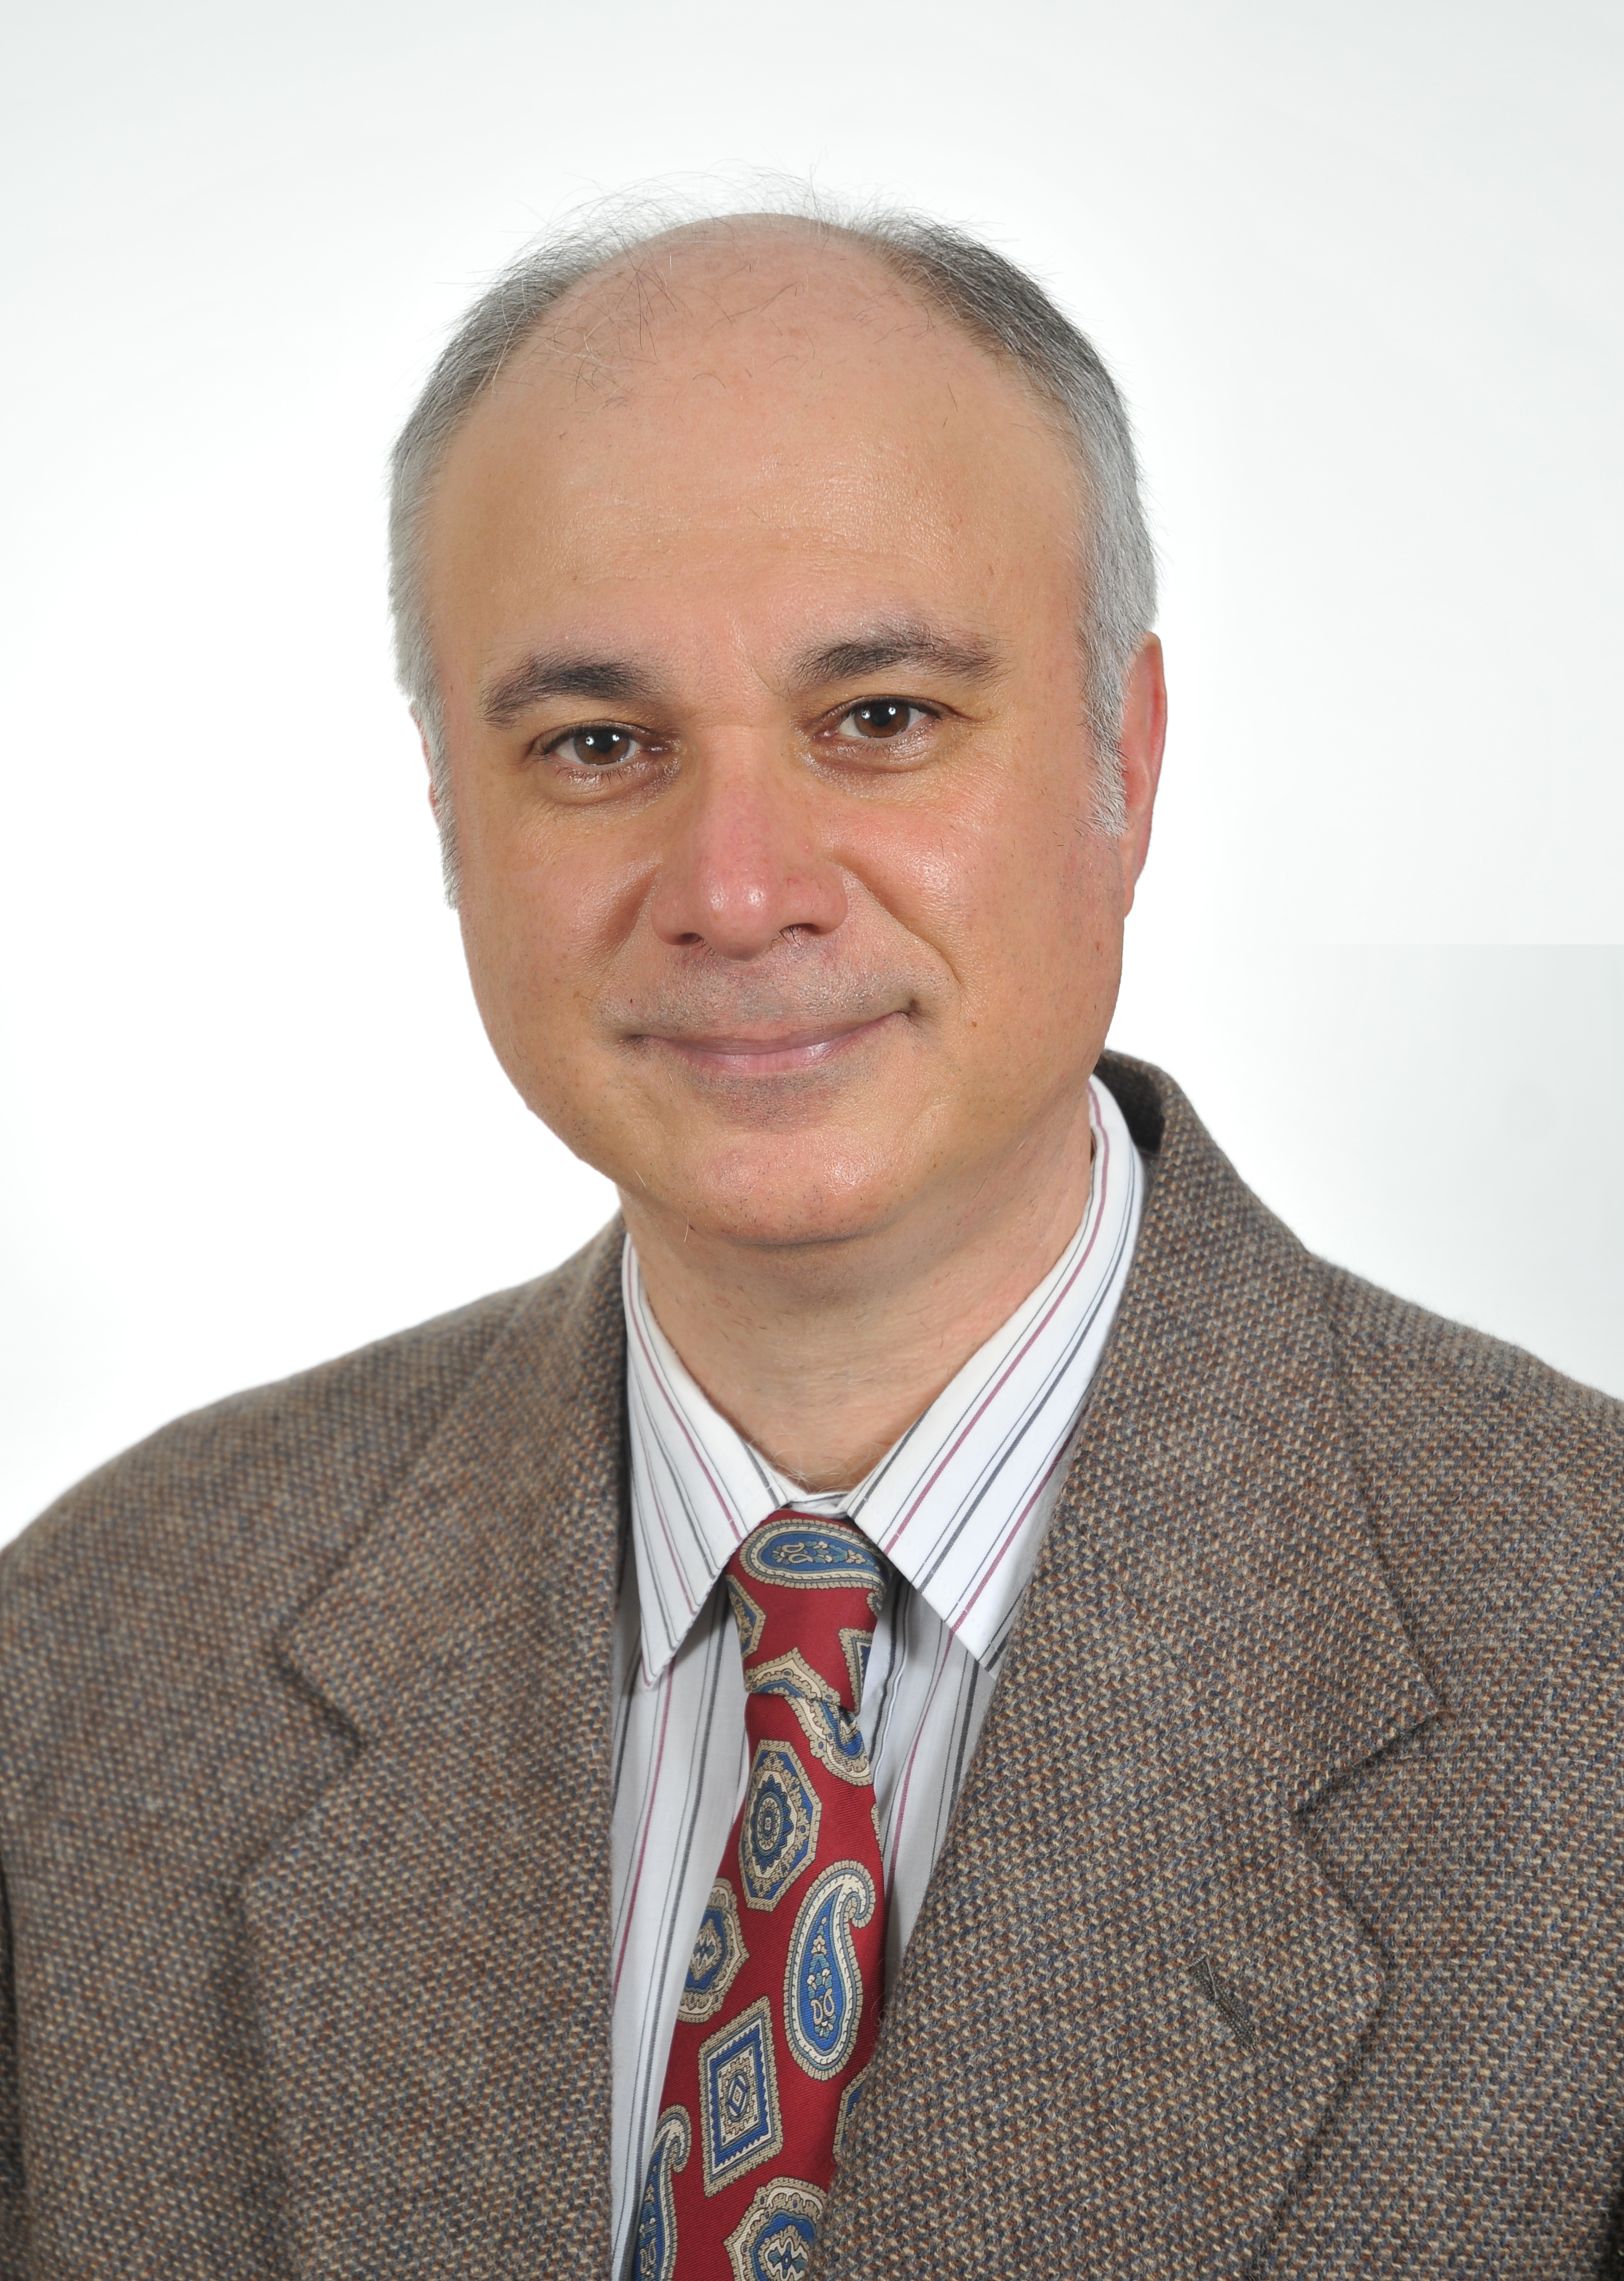
\includegraphics
[width=1in,height=1.25in,clip,
keepaspectratio]{images/jacob.jpg}}]
{Jacob Scharcanski}
received the B.Sc. degree in electrical engineering in 1981 and the M.Sc.
degree in computer science in 1987, both from the Federal University of Rio
Grande do Sul (UFRGS), Brazil, and the Ph.D. degree in systems design
engineering from the University of Waterloo, Canada, in 1993. Currently, he
is a Full Professor in computer science at UFRGS.  He has authored and
co-authored over 170 refereed journal and conference papers, and has
contributed to several books on imaging and measurements. In addition to his
academic publications, he has several technology transfers to the private
sector. Presently, he serves as an Associate Editor for two journals and has
served on dozens of International Conference Committees. Prof. Scharcanski is
a Senior Member of the IEEE, and served as an IEEE IMS Distinguished Lecturer
in several occasions. His areas of expertise are Image Processing, Pattern
Recognition, Imaging Measurements and Computational Methods in Finance.
\end{IEEEbiography}

\EOD

\end{document}
